\documentclass[8pt]{extarticle} 
\usepackage{graphicx} % Required for inserting images
\usepackage{amsfonts}
\usepackage{enumitem}
\usepackage[hidelinks]{hyperref}
\usepackage{graphicx}
\usepackage{textcomp}
\usepackage{amsmath}
\usepackage{multicol}
\usepackage{mathabx}
\usepackage[bottom=0.5cm, right=1.5cm, left=1.5cm, top=1.5cm, headheight=16pt]{geometry}
\usepackage{amssymb}
\usepackage{amsthm}
\usepackage{amsmath}
\usepackage{physics}
\usepackage{cancel}
\usepackage{mathtools}
\usepackage{array}
\usepackage{tikz}
\def\checkmark{\tikz\fill[scale=0.4](0,.35) -- (.25,0) -- (1,.7) -- (.25,.15) -- cycle;} 
\makeatletter
\newcases{crcases}{\quad}{%
  \hfil$\m@th\displaystyle{##}$\hfil}{\hfil$\m@th\displaystyle{##}$}{\lbrace}{.}
\makeatother
\usepackage{mdframed}
\usepackage{tikzlings}
\usepackage{tikzducks}
\usepackage{MnSymbol}
\usepackage{animate}
\usepackage{physics}



\title{\textbf{Fundamental Theorem of Calculus}}
\author{\textbf{Connor Li}}
\date{\textbf{March 2024}}

\newmdenv{boxedsection}

\begin{document}

\maketitle


\section*{Contact Information}
\begin{itemize}
    \item \underline{Author}: Connor Li
    \item \underline{Email}: connor.li@columbia.edu
    \item \underline{Phone Number}: (404) 642-6292
    \item \underline{LinkedIn}: \href{https://www.linkedin.com/in/connor-li-4871a71a9/}{Click Here}
    \item \underline{Personal Website}: \href{https://connorli18.github.io/}{Click Here}
    \item \underline{GitHub}: \href{https://github.com/connorli18}{Click Here}
    \item \underline{Resume}: \href{https://drive.google.com/file/d/1G4QryPZy70d9OCKWtcJPA6su5gIfjmIe/view?usp=sharing}{Click Here}
\end{itemize}
\vspace{2cm}
\tableofcontents

\pagebreak
\section{Overview}
\subsection{The Goal}
The goal of this document is to provide a comprehensive overview of the Fundamental Theorem of Calculus from both an analytical and practical standpoint. The content of the document will hopefully tie together important proofs, concepts, and give you a nice reminder/refresher over one of the most important concepts ever introduced in higher-level mathematics.
\subsection{Top Level}
The Fundamental Theorem of Calculus is a cornerstone in mathematics, linking two principal concepts: differentiation and integration. It highlights that differentiation and integration are inverse processes of each other. This theorem underpins the ability to compute the area under a curve using antiderivatives, illustrating a deep and intrinsic connection between rates of change (differential calculus) and accumulation of quantities (integral calculus). Essentially, it provides a comprehensive framework that allows for the practical application of calculus in solving real-world problems, by demonstrating how these seemingly disparate concepts are fundamentally intertwined.
\section{Establishing a Basis}
\subsection{The Derivative}
\subsubsection{Introduction}
If you've taken any math class, you're probably familiar with the concept of slope. Whether you've been taught it as ``rise over run'' or ``change in $y$ over change in $x$'', the concept is the same for lines. Intuitively, it tells you how fast a line is changing at a given point. But, not every interesting graph is a line, and oftentimes the graphs that we are interested in do not have constant slope. Take this function, for example.
\vspace{0.5cm}
$$
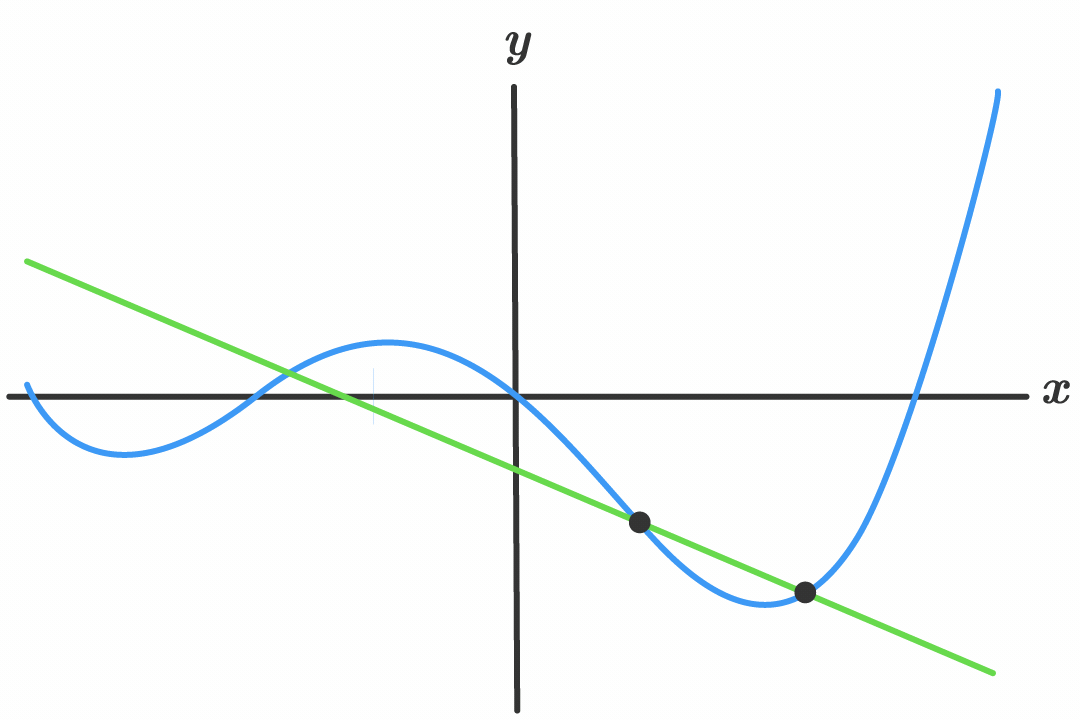
\includegraphics[width=6cm]{images/slope-0.png} \quad \quad \quad \quad 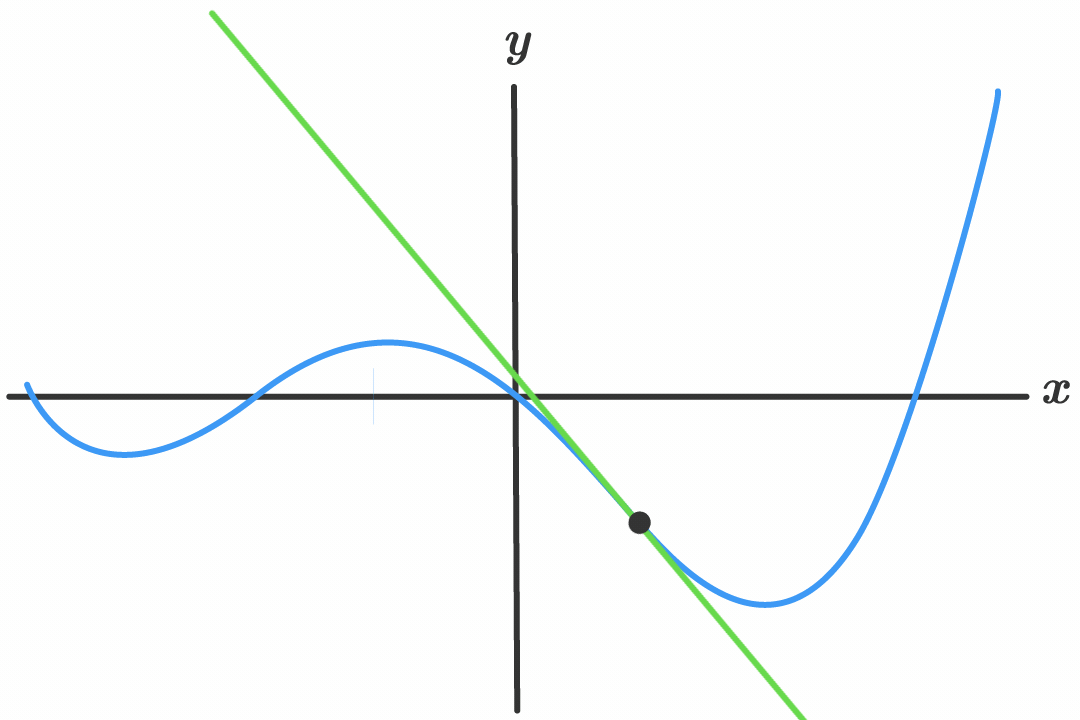
\includegraphics[width=6cm]{images/slope-132.png}
$$
As you can clearly see, at every point, the slope of the function is changing. So, we formalize our definition of the derivative as the instantaneous rate of change of a function at a given point. Basically, if you take tangent lines (lines that touch the graph at only one point) at every point on the graph, the slope of those lines is the derivative at the respective point.
\subsubsection{The Definition}
Using the intuition provided above, we can formally define the derivative of a function at any given point. Essentially, we can pick any two points of the function and take the slope of the line connecting them. And, as we decrease the distance that separates the two points, the slope of the line connecting them will approach the slope of the tangent line at the point. So, we present the following definition.
\begin{boxedsection}
\textbf{Definition (Derivative at a Point)}: Let $f(x)$ be any function. Then, we can say the derivative of $f(x)$ at any point $a$ (if it exists), which we will denote $f'(a)$, is defined by
$$
f'(a) = \lim_{x \rightarrow a} \frac{f(x) - f(a)}{x-a} = \lim_{h \rightarrow 0} \frac{f(a+h) - f(a)}{h}
$$
\underline{Note}: These definitions are the same under the change of variables $h = x -a$. 
\end{boxedsection}
If $f'(a)$ exists and is well defined at every point in the function's domain, then we can say that there exists some function $f'(x)$ that represents the derivative at every point. This is the case for most functions that we encounter in practice, and we call this function $f'(x)$ the derivative of $f(x)$.
\begin{boxedsection}
\textbf{Definition (Derivative of a Function):} A function $f(x)$ is called differentiable at $x=a$ if $f'(a)$ exists and is called differentiable on an interval if it is differentiable at every point in the interval. The function $f'(x)$ is called the derivative of $f(x)$.
\end{boxedsection}
\subsection{The Integral}
\subsubsection{Introduction}
The integral is a concept related to find ``the area under the curve''. Very generally, the concept relies on taking ``boxes'' of some width where the height of the boxes are defined by the function $f(x)$. If you add these boxes together, you get an approximation of the area under the curve.
$$
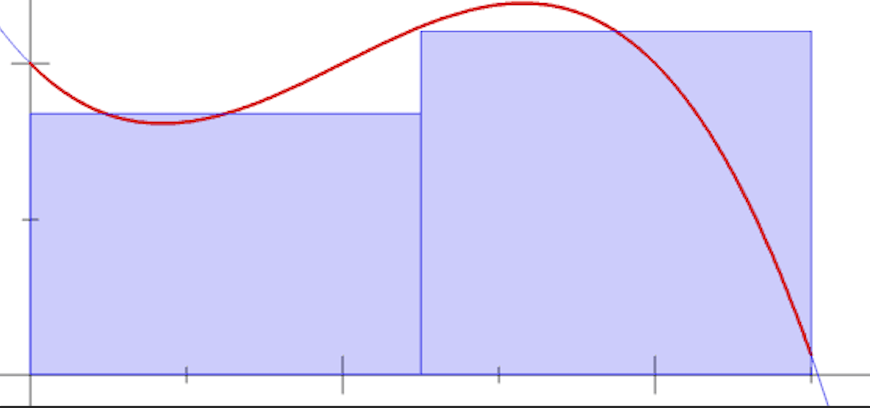
\includegraphics[width=7cm]{images/part1integral.png} \quad \quad \quad \quad
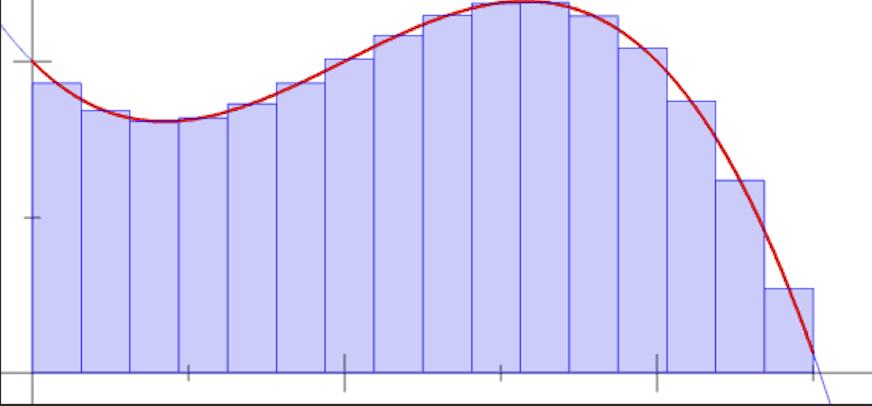
\includegraphics[width=7cm]{images/part2integral.png}
$$
The method of taking these boxes is demonstrated in the pictures above. If you notice, the approximation gets better as the width of the boxes decreases. This is because the approximation gets closer to the actual area under the curve. So, we can formally define the integral as the limit of these approximations.
\subsubsection{The Definition}
The definite integral from $a$ to $b$ of a function $f(x)$ is ``the area under the curve'' of $f(x)$ from point $a$ to point $b$, which we denote as follows.
$$
\int_a^b f(x) \;dx
$$
In this case, the $dx$ is what we call the ``term of integration,'' which is a notation that tells us that we are integrating with respect to $x$ (i.e. finding the area with respect to a change in $x$). Using the intuition above, we can define the definite integral as follows.
\begin{boxedsection}
  \textbf{Definition (Definite Integral):} Let $f(x)$ be any function over the interval $x \in [a,b]$. If we divide $[a,b]$ into $n$ subintervals of equal width $(\Delta x)$, and pick any point over each divided interval $x_i^*$, then the definition integral is defined as follows.
  $$
  \int_a^b f(x) \;dx = \lim_{n\rightarrow\infty} \sum_{i=1}^n f(x_i^*) \Delta x 
  $$
  \underline{Note}: In this case, we are taking $n$ of these small intervals where the width of the mini-rectangle is $\Delta x$ and the height of said rectangle is $f(x_i^*)$. Since we take $n \rightarrow \infty$, we are adding up more and more rectangles to get a better (almost perfect) approximation of the area under the curve.
\end{boxedsection}
Now, you're probably wondering about indefinite integrals. Like derivatives, we are interested in the expression $\int f(x)\;dx$ without bounds. Specifically, we want to know if it's possible to express the indefinite integral as a function of $x$. To answer this question, we must use the Fundamental Theorem of Calculus, which we will discuss in the next section.
\pagebreak
\section{Precursors to the Theorem}
\subsection{Overview}
To rigorously prove the Fundamental Theorem of Calculus and elucidate the deep-seated connection between the operations of integration and differentiation, it is imperative to invoke a suite of fundamental theorems. This methodology serves not only to validate the theorem itself but also to illuminate the inherent linkage between integration and differentiation, thereby providing a solid foundation for a substantial portion of calculus theory. The subsequent discussion will employ analytical techniques useful in any higher-level proofs course.
\subsection{Intermediate Value Theorem}
The Intermediate Value Theorem is another fundamental theorem in calculus that we will use to prove the Mean Value Theorem. Intuitively, the theorem states that if a function is continuous on a closed interval $[a,b]$, then the function must attain every value between $f(a)$ and $f(b)$ over the interval $[a,b]$. The proof is quite complicated, and will be left via link.
\begin{boxedsection}
  \textbf{Theorem:} If $f$ is a continuous function on $[a,b]$ and $k$ is any number between $f(a)$ and $f(b)$, then there exists some $c \in (a,b)$ where $f(c) = k$.\\
  \\
  \textbf{Proof:} The proof is quite complex (and uses techniques from analysis), but a version of it is linked \href{https://math.oxford.emory.edu/site/math111/proofs/ivt/}{here}. 
\end{boxedsection}
\subsection{Extreme Value Theorem}
The Extreme Value Theorem is a fundamental theorem in calculus that we will use to prove the Fundamental Theorem of Calculus.
Intuitively, the theorem is quite simple. It states that if a function is continuous on a closed interval $[a,b]$, then the function must attain some maximum and minimum value over the interval $[a,b]$.
\begin{boxedsection}
  \textbf{Theorem:} If $f$ is continuous function over the closed, bounded interval of $[a,b]$, then $f$ attains some maximum and minimum value over the interval $[a.b]$.\\
  \\
  \textbf{Proof:} The proof is quite complex, but a version of it is linked \href{https://mathcenter.oxford.emory.edu/site/math111/proofs/extremeValueTheorem/}{here}.
\end{boxedsection}
This will be used as a counterpart to prove the Mean Value Theorem, which is another important theorem that we will use to prove the Fundamental Theorem of Calculus.
\subsection{Mean Value Theorem}
The Mean Value Theorem is another important building block to the Fundamental Theorem of Calculus. It states that if a function is continuous on a closed interval $[a,b]$ and differentiable on the open interval $(a,b)$, then there exists some point $c \in (a,b)$ such that the derivative at $c$ is equal to the average rate of change of the function over the interval. More intuitively, it's saying that there exists some point whose derivative is the average rate of change.
\begin{boxedsection}
\textbf{Theorem (Mean Value):} If $f$ is continuous on the closed interval $[a,b]$ and differentiable on $(a,b)$, then there is at least one point $c \in [a,b]$ such that
$$
f(c) = \frac{1}{b-a} \int_a^b f(x)\;dx \quad \quad \text{ or } \quad \quad f(c)(b-a) = \int_a^b f(x)\;dx
$$
\textbf{Proof:} Since $f(x)$ is continuous on the closed interval, we can use the extreme value theorem to show that $f(X)$ attains some maximum $M$ and minimum $m$ over that interval. This means that for all $x \in [a,b]$, we have that $m \leq f(x) \leq M$. Thus, since the integral is the area under the curve, we can construct the comparison rectangles and show the bounds
$$
m(b-a) \leq \int_a^b f(x)\;dx \leq M(b-a) \implies m \leq \frac{1}{b-a} \int_a^b f(x)\;dx \leq M
$$
Since our term $\frac{1}{b-a} \int_a^b f(x)\;dx$ is bounded and $f(x)$ is continous over the interval and assumes values $M$ and $m$, we can use the intermediate value  theorem to show that there exists some $c \in [a,b]$ such that
$$
f(c) = \frac{1}{b-a} \int_a^b f(x)\;dx
$$
This completes the proof.
\end{boxedsection}
Although this is more complicated (and requires \href{https://mathcenter.oxford.emory.edu/site/math111/proofs/rollesTheorem/}{Rolle's Theorem}), a corollary of this theorem above tells us the following result.
\begin{boxedsection}
  \textbf{Corollary (Mean Value)}: Let $f$ be continuous over the closed interval $[a,b]$ and differentiable over the open interval $(a,b)$. Then, there exists one point $c \in (a,b)$ such that
  $$
  f'(c) = \frac{f(b)-f(a)}{b-a}
  $$
  \textbf{Proof:} The proof will be left as an exercise.
\end{boxedsection}
\pagebreak
\section{The Fundamental Theorem of Calculus}
\subsection{Overview}
The Fundamental Theorem of Calculus ties together the integration and differentiation of functions. 
It is composed of two parts, the first of which establishes the relationship between differentiation and integration. The second part is arguable even more important, giving us a more holistic definition of integration in terms of an anti-derivative function!
\subsection{Part 1}
Before we begin the proof, I think that it's important to mention notationally that $F(x)$ is defined as the anti-derivative of $f(x)$. In most situations, we see the definite integral as a number, but the Fundamental Theorem of Calculus allows us to see the definite integral as a function of $x$. This is because one of the bounds is some variable $x$ instead of a fixed point, which introduces the first part of the theorem.
\begin{boxedsection}
\textbf{Theorem:} If $f(x)$ is continuous on an interval $[a,b]$, and the function $F(x)$ is defined as follows
$$
F(x) = \int_a^x f(t)\;dt
$$
Then, $F'(x) = f(x)$ over $[a,b]$. \\
\\
\textbf{Proof:} If we use the definition of the derivative on $F(x)$ and its definition as the integral, we have the following theorem.
\begin{align*} 
  F'(x) &= \lim_{h\rightarrow 0} \frac{F(x+h) - F(x)}{h}\\
  &= \lim_{h\rightarrow 0} \frac{1}{h} \left[\int_a^{x+h} f(s)\;ds - \int_a^x f(x)\;ds \right]\\
  &= \lim_{h\rightarrow 0} \frac{1}{h} \left[\int_a^{x+h} f(s)\;ds + \int_x^a f(x)\;ds \right]\\
  &= \lim_{h\rightarrow 0} \underbrace{\frac{1}{h} \int_x^{x+h} f(s)\;ds}_{\Lambda}
\end{align*}
The term $\Lambda$ is just the average value of $f(s)$ over the interval $[x,x+h]$. This allows us to use the Mean Value Theorem from above to say that there exists some $c \in [x,x+h]$ such that $f(c) = \Lambda = \frac{1}{h} \int_x^{x+h} f(s)\;ds$.
However, since we are taking the limit as $h \rightarrow 0$, this means that $c \rightarrow x$ since $c$ is between $x$ and $x + h$. Finally, using the property of continuity for $f(x)$, we have the following result.
$$
\lim_{h\rightarrow 0} \frac{1}{h} \int_x^{x+h} f(s)\;ds = \lim_{c \rightarrow x} f(c) = f(x)
$$
This completes the proof that $F'(x) = f(x)$ over $[a,b]$.
\end{boxedsection}
If you couldn't tell from the name, the Fundamental Theorem of Calculus has a lot of implications. It not only proves the relationship between derivation and integration, but it also proves that every integrable function has an anti-derivative function, as as a corrollary, that any continuous function has a well-defined anti-derivative.
\subsection{Part 2}
The second part of the Fundamental Theorem of Calculus is also known as the evaluation theorem. The general intuition behind the formula is that the definite integral of a function $f(x)$ is equal to the anti-derivative evaluated at only endpoints of the interval. In a more general sense, it eliminates the need to keep taking smaller boxes since we can find the area under the curve by evaluating the anti-derivative function.
\begin{boxedsection}
  \textbf{Theorem:} If $f(x)$ is continuous on an interval $[a,b]$ and $F(x)$ is the antiderivative of $f(x)$, then
$$
  \int_a^b f(x)\;dx = \eval{F(x)}_a^b = F(b) - F(a)
$$
\textbf{Proof:} Let's first divide $[a,b]$ into $n$ continuous segments of equal length and label the endpoints of each segment $x_i$ where $i = 0,\;1,\;\dots,\;n$. This means that our interval $[a,b]$ now looks like
$$
[a,b] = [x_0,x_1] \cup [x_1,x_2] \cup \dots \cup [x_{n-1},x_n]
$$
This means that we can rewrite the expression $F(b) - F(a)$ as follows.
\begin{align*}
F(b) - F(a) &= F(x_n) - F(x_0)\\
&=  \left[F(x_n) - F(x_{n-1})\right] + \left[F(x_{n-1}) - F(x_{n-2})\right] + \dots + \left[F(x_1) - F(x_0)\right]\\
&= \sum_{i=1}^n \left[F(x_i) - F(x_{i-1})\right]
\end{align*}
Now, we can use the Mean Value Theorem (corollary) for every interval $[x_{i-1}, x_i]$ to say that there exists some $c_i \in (x_{i-1},x_i)$ such that
$$
F'(c) = \frac{F(x_i) - F(x_{i-1})}{x_i - x_{i-1}} \implies F(x_i) - F(x_{i-1}) = F'(c_i)(x_i - x_{i-1}) = f(c_i)(x_i - x_{i-1}) = f(c_i)\Delta x
$$
And, as we take the limit as $n \rightarrow \infty$ for our original expression, we have
$$
F(b) - F(a) = \lim_{n\rightarrow \infty} \sum_{i=1}^n f(c_i) \Delta x = \int_a^b f(x)\;dx 
$$
\end{boxedsection}
\subsection{Part 3}
If you aren't interested in Calculus III/IV concepts, please skip this section. But if you are, the Fundamental Theorem of Calculus has an extension to integrals along curves (path integrals). 
\begin{boxedsection}
  \textbf{Theorem:} If $f(z)$ has a continuous indefninite integral $F(z)$ in a region $R$ with the parameterized curve $\gamma: z = z(t)$ for all $t \in [a,b]$, then
  $$
  \int_\gamma f(z)\;dz = F(z(b)) - F(z(a))
  $$
  \textbf{Proof:} The proof is quite complex, and I don't think it's very valuable to look at. However, the intuition remains the same, that the integral of a function along a curve is equal to the anti-derivative evaluated at the endpoints of the curve.
\end{boxedsection}

\subsection{Example Problems}
\subsubsection{FTC Part 1}
\textbf{Problem (1):} Find the derivative of the following function.
$$
g(x) = \int_1^x \frac{1}{t^3 + 1}\;dt
$$
\textbf{Problem (2):} Find the derivative of the following function.
$$
g(x) = \int_x^{x^2} t^3 \;dt
$$
\subsubsection{FTC Part 2}
\textbf{Problem (1):} Evaluate the following definite integral.
$$
\int_{-2}^2 \frac{t^3}{3} - 4 \;dt 
$$
\textbf{Problem (2):} Evaluate the following definite integral.
$$
\int_{1}^9 \frac{x-1}{\sqrt{x}}\;dx
$$
\end{document}
